\documentclass[11pt]{report}
% packages
% Fran Burstall's Bath thesis package
\usepackage{baththesis}
\usepackage{amssymb} %for Blackboard bold etc \usepackage{graphicx} %for including eps graphics % front matter
\usepackage[pdftex]{graphicx} % To include pictures
\usepackage{caption}
\usepackage{subcaption} % To use subfigures with subcaptions
\usepackage{url}
\usepackage{amsmath} % Equations
\usepackage{txfonts}
\setlength{\parskip}{0.9em} %Paragraph spacing
\usepackage{pgfgantt}
\usepackage{cite}
\usepackage{csquotes}
\usepackage{multirow}
\usepackage{hhline} % Double lines in tables
\usepackage[ruled]{algorithm2e} % Algorithms 
\renewcommand*{\mkcitation}[1]{ #1}
\usepackage{listings} % For C++ code
\lstset{language=C++,
                basicstyle=\scriptsize,
                keywordstyle=\color{blue}\ttfamily,
                stringstyle=\color{red}\ttfamily,
                commentstyle=\color{green}\ttfamily,
                morecomment=[l][\color{magenta}]{\#},
                showstringspaces=false
}

\newcommand{\phim}{\mathbf{\phi}}
\newcommand{\X}{\mathbf{X}}
\newcommand{\x}{\mathbf{x}}
\newcommand{\Y}{\mathbf{Y}}
\newcommand{\y}{\mathbf{y}}
\newcommand{\w}{\mathbf{w}}
\newcommand{\Z}{\mathbf{Z}}
\newcommand{\z}{\mathbf{z}}
\newcommand{\h}{\mathbf{h}}
\newcommand{\omegam}{\boldsymbol{\omega}}
\newcommand{\deltax}{\left \|  \Delta x \right \|}
\newcommand{\lxo}{\lambda, \x, \omegam}
\newcommand{\C}{\,^{\circ}{\rm C}}
\newcommand{\Maya}{Maya\textsuperscript\textregistered~}
\newcommand{\MentalRay}{Mental Ray\textsuperscript\textregistered~}
\newcommand{\Matlab}{Matlab\textsuperscript\textregistered~}

%\usepackage[hidelinks]{hyperref} % Adds references links without color
\usepackage{hyperref} % Adds references links with color
\usepackage{xcolor}
\hypersetup{
    colorlinks,
    linkcolor={red!50!black},
    citecolor={blue!50!black},
    urlcolor={blue!80!black}
}

\DeclareMathOperator*{\argmin}{arg\,min}
\DeclareMathOperator*{\argmax}{arg\,max}

\title{Realistic fire rendering} \author{Garoe Dorta-Perez}
%\degree{Doctor of Philosophy}
\unit{ CM50170 - Research project }
\department{} 
\degreemonthyear{August 2015}
\norestrictions

% Write here the section you are working on to compile only that one
% You can write more than one section separated by comma
% Comment to compile all
% \includeonly{conclusions} 


\begin{document}

\maketitle

{\hypersetup{linkcolor=black} % Set color back to black
\tableofcontents
}

%------------------------------------------------------------------------------
\chapter{Introduction}
\label{ch:introduction}
\textquote{\textit{A case that can be made for fire being, next to the life process, the most
complex of phenomena to understand}.} - Hoyt Hottle

\begin{figure}[htpb!]
        \centering
        \begin{subfigure}[t]{0.25\textwidth}
                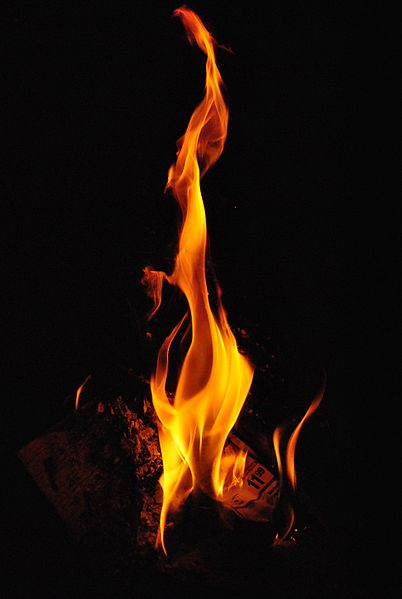
\includegraphics[width=\textwidth]{img/real_fire1}
                \caption{Paper fire~\cite{real_fire1}.}
                \label{fig:real_fire1}
        \end{subfigure}%
        ~ %add desired spacing between images, e. g. ~, \quad, \qquad, \hfill etc.
          %(or a blank line to force the subfigure onto a new line)
        \begin{subfigure}[t]{0.55\textwidth}
                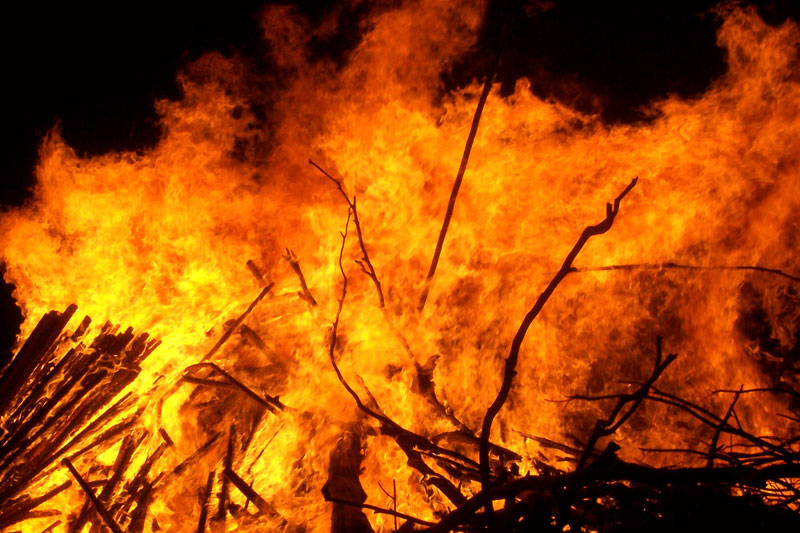
\includegraphics[width=\textwidth]{img/real_fire2}
                \caption{Bone fire~\cite{real_fire2}.}
                \label{fig:real_fire2}
        \end{subfigure}
        \caption{Examples of real fire.}\label{fig:real_fires}
\end{figure}

Computer simulations are widely used to model a diverse range of natural phenomena.
Their popularity lies in their inexpensive nature, predictive capabilities given good mathematical models, parameters can be changed at will to produce new results, the equations governing the system can be modified to create scenarios that are not physically attainable, etc.
Computer generated graphics are used to display the results of the simulations.
Rendering the data on the screen involves transforming a scene into an image that can be displayed using some light transport and illumination model.

For centuries humans has been attracted to fire due to its attractive presence and its dangerous nature, real fire examples are shown in Figure~\ref{fig:real_fires}.
Combustion phenomena are prevalent in daily life, candles, camp fires, explosions, car engines, cooking appliances, etc.
Simulating and visualizing fire related processes has many applications, for example it is widely used for visual effects in the film industry, simulated as part of the virtual environment in the computer games industry; or in the engineering community, where modelling engine combustion and fire safety evaluations are frequently demanded.

Computer generated examples in films include, a planet explosion in Star Trek II, as shown in Figure~\ref{fig:reeves_1983}, where a particle-based technique by~\cite{Reeves:1983} was used; Shrek featured a dragon exhaling fire, as shown in Figure~\ref{fig:lamorlette_2002}, where parametric curves were used to drive the flames~\cite{Lamorlette:2002}; or the more recent work of~\cite{Horvath:2009} based on 2D screen projections for the film Harry Potter and the Deathly Hallows, as shown in Figure\ref{fig:horvarth_2009}.
In these and in many other applications, using real flames is an expensive and hazardous endeavour.

\begin{figure}[htpb!]
        \centering
        \begin{subfigure}[b]{0.3\textwidth}
                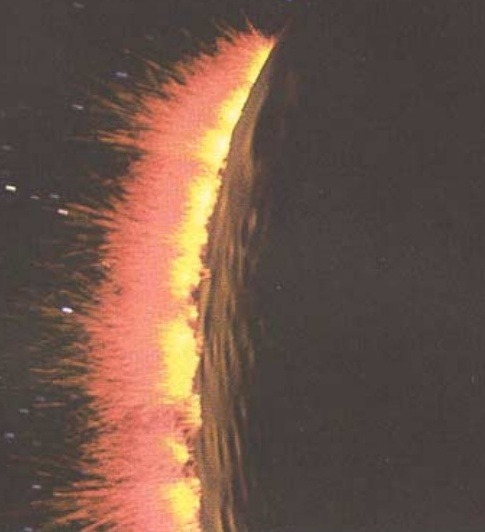
\includegraphics[width=\textwidth]{img/reeves_1983}
                \caption{Explosion in Star Trek II~\cite{Reeves:1983}.}
                \label{fig:reeves_1983}
        \end{subfigure}%
        \quad %add desired spacing between images, e. g. ~, \quad, \qquad, \hfill etc.
          %(or a blank line to force the subfigure onto a new line)
        \begin{subfigure}[b]{0.5\textwidth}
                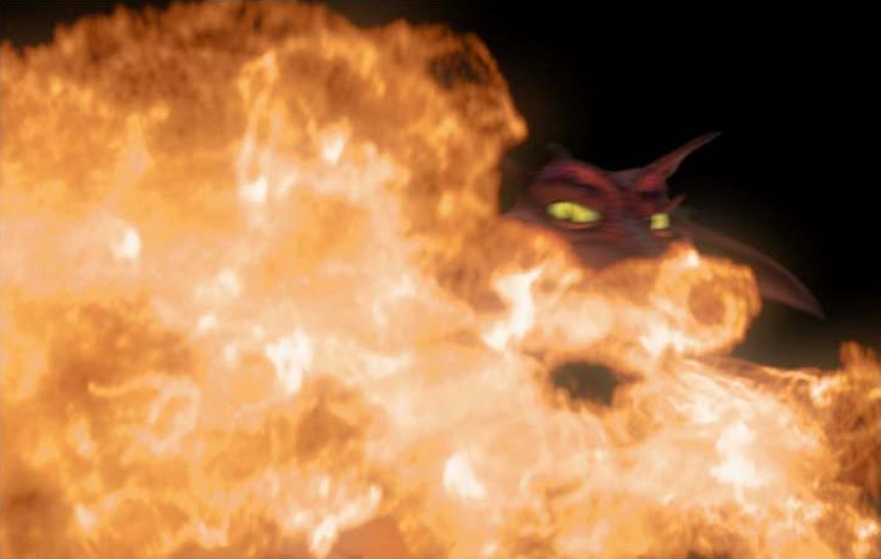
\includegraphics[width=\textwidth]{img/lamorlette_2002}
                \caption{Dragon fire in Shrek~\cite{Lamorlette:2002}.}
                \label{fig:lamorlette_2002}
        \end{subfigure}
        ~ %add desired spacing between images, e. g. ~, \quad, \qquad, \hfill etc.
          %(or a blank line to force the subfigure onto a new line)
        \begin{subfigure}[b]{0.5\textwidth}
                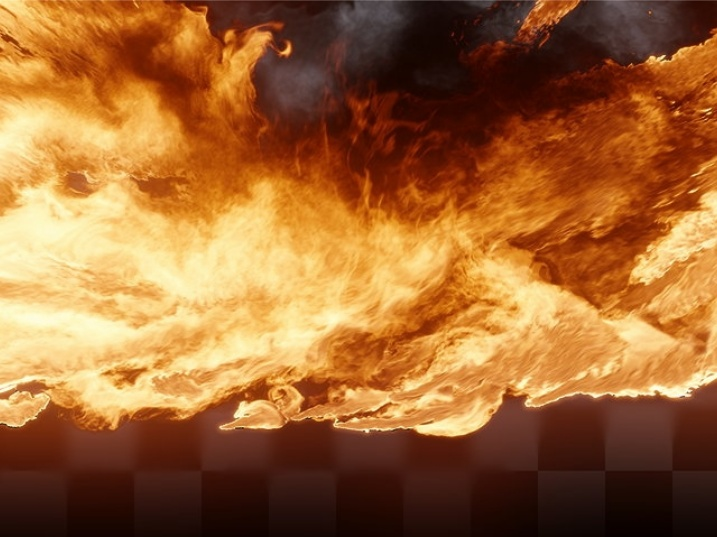
\includegraphics[width=\textwidth]{img/horvarth_2009}
                \caption{Flames used in Harry Potter and the Deathly Hallows~\cite{Horvath:2009}.}
                \label{fig:horvarth_2009}
        \end{subfigure}
        \caption{Examples of visual effects with fire in the film industry.}
\end{figure}


The computer graphics community have intensively researched the fluid behaviour of water and smoke.
Fire can be also be modelled as a fluid, however due to its multiphase flow, chemical reactions and radiative heat transport, the techniques used for water or smoke cannot be directly applied to flames.
As a result of the aforementioned complexity and the interdisciplinary nature of the problem, fire simulation is still an open problem in computer graphics.

A great deal of work done in the area has sacrificed complexity for interactiveness, therefore producing simplified models which hope to deceit the observer by exploiting the chaotic behaviour present in fire motion.
Nevertheless, physically-based simulations incorporate the intrinsic processes that occur in a combustion scenario in order to be able to produce realistic results.
In general the following effects are taken into consideration

\begin{description}
\item[Flame motion:] under normal gravity conditions, convection, external wind forces, front propagation and gas expansion drive the shape and position of the flame. 
\item[Fuel erosion:] when the fuel reaches a certain temperature, it is vaporized into a gaseous state, which rises under the influence of buoyancy.
\item[Flame colour:] the chemical species present in the fuel and the byproducts of the combustions emit energy in various wavelengths due to black body radiation.
\end{description}

In this report a short review of fire simulation and rendering methods is presented in Chapter~\ref{ch:previous_work}.
In Chapter~\ref{ch:methodology}, a state-of-the-art physically-based model to render fire, proposed by ~\cite{Pegoraro:2006}, is discussed extensively.
Implementation details of a \MentalRay shader for the the given model are outlined in Chapter~\ref{ch:previous_work}, and results are discussed in Chapter~\ref{ch:results}.
Lastly, conclusions and future research directions are considered in Chapter~\ref{ch:conclusions}.

%------------------------------------------------------------------------------
\chapter{Previous Work}
\label{ch:previous_work}

In order to display a realistic fire scene in a computer generated world two differentiated stages are needed.
Firstly, the fire dynamics have to be collected, this can either be done through a data capture session or simulated using a fluid solvers.
Secondly, the previously gathered data is to be visualized on the screen using some rendering technique.
We refer the interested readers to the more detailed survey on the topic, which has been recently presented by~\cite{Huang:2014}.

\section{Simulation}
\label{sec:simulation}

%\section{Fire Simulation}
%\label{sec:fire_simulation}

\textbf{Particle-based methods} were the first approach to simulate the visual animation of fire.
A number of particles are emitted from certain locations, each particle has a set of attributes such as shape, velocity, color or lifetime.
The first model with particle systems was presented by~\cite{Reeves:1983}, the particles speed and colour were perturbed with a Gaussian noise at each time step, and the colour was subject to an additional linear perturbation on its lifetime.
Two particle systems were used in a hierarchy, one would control fire spread and the other a single explosion effect.
An extension was proposed by~\cite{Perry:1994}, the authors modified the particle system such that each particle shape would be defined by a series of non-overlapping coplanar triangles.
The transparency of would increase towards the outer vertices, thus providing an improved visual effect.


\textbf{Noise-based methods} focus on synthesizing the high fluctuation present in fire procedurally.
The objective is to approximate the turbulence present in fire with an appropriate statistical model.
Using a variation of Perlin noise, ~\cite{Perlin:1985} presented images of a corona of flames.
However, the method is limited to 2D, where the color is a combination of non-linear arbitrary functions.
This work was extended by~\cite{Perlin:1989} to 3D, where they use volumetric rendering to achieve improved results.

\textbf{Geometry skeleton}

\textbf{Data driven}

\textbf{Physically based} simulate the fire combustion processes, including flame propagation or the chemical reactions that convert fuel into gaseous products.  
Incompressible flow equations were used by~\cite{Stam:1995} to drive a fire simulation.
Given initial fuel conditions, the fire spread is advected on a grid using an advection-diffusion type equation.
Building on the work on a semi-Lagrangian fluid solver of~\cite{Stam:1999}, a model which includes gaseous fuel and gaseous byproducts was proposed by~\cite{Nguyen:2002}.
In order to include the characteristics of the noise-based methods, \cite{Hong:2007} combined the previous model with a set of third-order equations from detonation shock dynamics presented by~\cite{Yao:1996}.
As with the noise-based methods, this addition is visually attractive, yet it is not physically based. 
Capitalizing on the recent advances in GPUs parallel processing power, \cite{Horvath:2009} proposed a fixed camera model.
Particle properties are computed on a three-dimensional coarse grid, which are then projected into several view dependant two-dimensional slices.
The authors' model is based on the assumption that fine variations, which are perpendicular to the projection plane, are not individually visible and, they do not affect significantly the overall flow.
 
\textbf{Other effects} directly related to fire have also been explored.
\cite{Feldman:2003} presented a model to simulate suspended particles during explosions.
An incompressible fluid model drives the motion of air and hot gases, and the suspended particles follow the their movements.
Sound is a important factor to increase the believability of a finished fire animation.
\cite{Chadwick:2011} proposed a method to automatically generate plausible noise given for a given fire simulation.
Low frequency sound is estimated using a physical model whose inputs are the flame front and heat release.
A data driven sound synthesis approach, based on the work by~\cite{Wei:2000}, is applied to generate the high frequency content.

\textbf{Erosion}???


%\subsection{Smoke Simulation}
%\label{sec:smoke_simulation}


\section{Rendering}
\label{sec:rendering}

Rendering fire is more challenging than rendering other type of participating media, the main reason being that fire is a light-emitting source.
The luminescence radiated by a flame is generated by black body radiation due to the high temperature of the particles present during the combustion.
In order to render fire realistically, light absorption and scattering in the media, including air, has to be taken into consideration.

\subsection{Raster-Based}
\label{sec:raster_based}

Raster-based techniques sacrifice quality in the interest of interactive frame rates.
Some form of texture mapping is usually practised, usually only the surface of the flame is considered, and the illumination of the scene is approximated base on some parameter which can be easily computed such as a as well, e.g. the fire height.

\cite{Reeves:1983} applied a linear colour assignment to each particle in their simulation based on their lifetime.
\cite{Lee:2001} applied the same technique to render fires on mesh surfaces, where a particle would begin with a light yellow colour, evolve to red and finish in black at the end of their lifetime.
\cite{Lamorlette:2002} presented a technique were a based flame picture is mapped onto the two-dimensional flame profile with a base colour.
For each particle an intermediate emitting value is computed, and the final colour is super-sampled profile from an approximation of the cross-sectional area of the flame, as it would appear from the camera.
\cite{Zhang:2011} proposed a method were fire particles and their attributes are first projected onto a set of slicing planes, which are orthogonal to the camera direction. 
The planes are then blended to the screen in back-to-front order, and a one-dimensional colour texture is used as transfer function to convert flow attributes to colours and opacities.


\subsection{Ray-Tracing-Based}
\label{sec:ray_tracing_based}

Volume ray-tracing techniques offer astonishing results, however the associated computational costs are considerable.
Rays are shot from the view plane and evaluated at small increments; the total radiance at origin of the ray is computed by integrating the radiance at each step size.
A further drawback for ray tracing techniques, in comparison to raster-based methods, is the lack of a standard ray-tracing pipeline.

\cite{Rushmeier:1995} presented a method to perform accurate ray casting on sparse measured data.
The fire was modelled as a series of stacked cylindrical rings, where each ring has with uniform properties.
The total radiance at each point is integrated using a MonteCarlo method, summing up the measured irradiances at sample locations. 
\cite{Nguyen:2002} proposed a ray marching technique to solve the Radiative Transport Equation, see Chapter~\ref{ch:methodology}.
The emitted light is computed using Planck's formula of black body radiation, the light scattering in the media and visual adaptation to the fire spectra are modelled.
\cite{Feldman:2003} also included black body radiation in their animation of fire with suspended particles, however the mapping to RGB was manually adjusted to match the images of real explosions.
Direct illumination shadows were computed using deep shadow maps~\cite{Lokovic:2000}, while scattering and illumination by other objects in the scene used the technique proposed by~\cite{Jensen:2002}.
An extension to~\cite{Nguyen:2002} was presented by~\cite{Pegoraro:2006}, the authors' model has physically-based abortion, emission and scattering properties.
The spectroscopy characteristics of different fuels are achieved by modelling the electronic transitions between states in the molecules.
Non-linear trajectories of light in the medium due to light refraction effects are included as well.
In order to minimize the effects induced by the limitations of the RGB colour space, the visual adaptation process is presented as a post-processing effect.
\cite{Horvath:2009} proposed a rendering method whose main objective was user-friedliness for artists.
Using the fixed camera slices described in Section~\ref{sec:simulation}, the authors' perform a simple volume rendering to join them in a single image.
Black body radiation is used for the light, the images are motion-blurred with a filter based on the velocities in the slices, and the heat distortion is added as post-processing user defined filter. 

%------------------------------------------------------------------------------
\chapter{Methodology}
\label{ch:methodology}

Given simulated or captured fire data, that could come from any of the methods discussed in Section~\ref{sec:simulation}, we want to generate a photo-realistic image from a camera view of the scene.
From this point onwards we will assume that we have a volumetric data structure, which holds the relevant input data for the fire.
An overview of the pipeline based on the work by \cite{Pegoraro:2006} is shown in Figure~\ref{fig:pipeline}.
The inputs are volumetric data of density and temperature, from those values a series of intermediate constants for each voxel for the current frame are computed, and with the previous data a ray marcher is used to generate the final image.

\begin{figure}[htbp!]
	\centering
	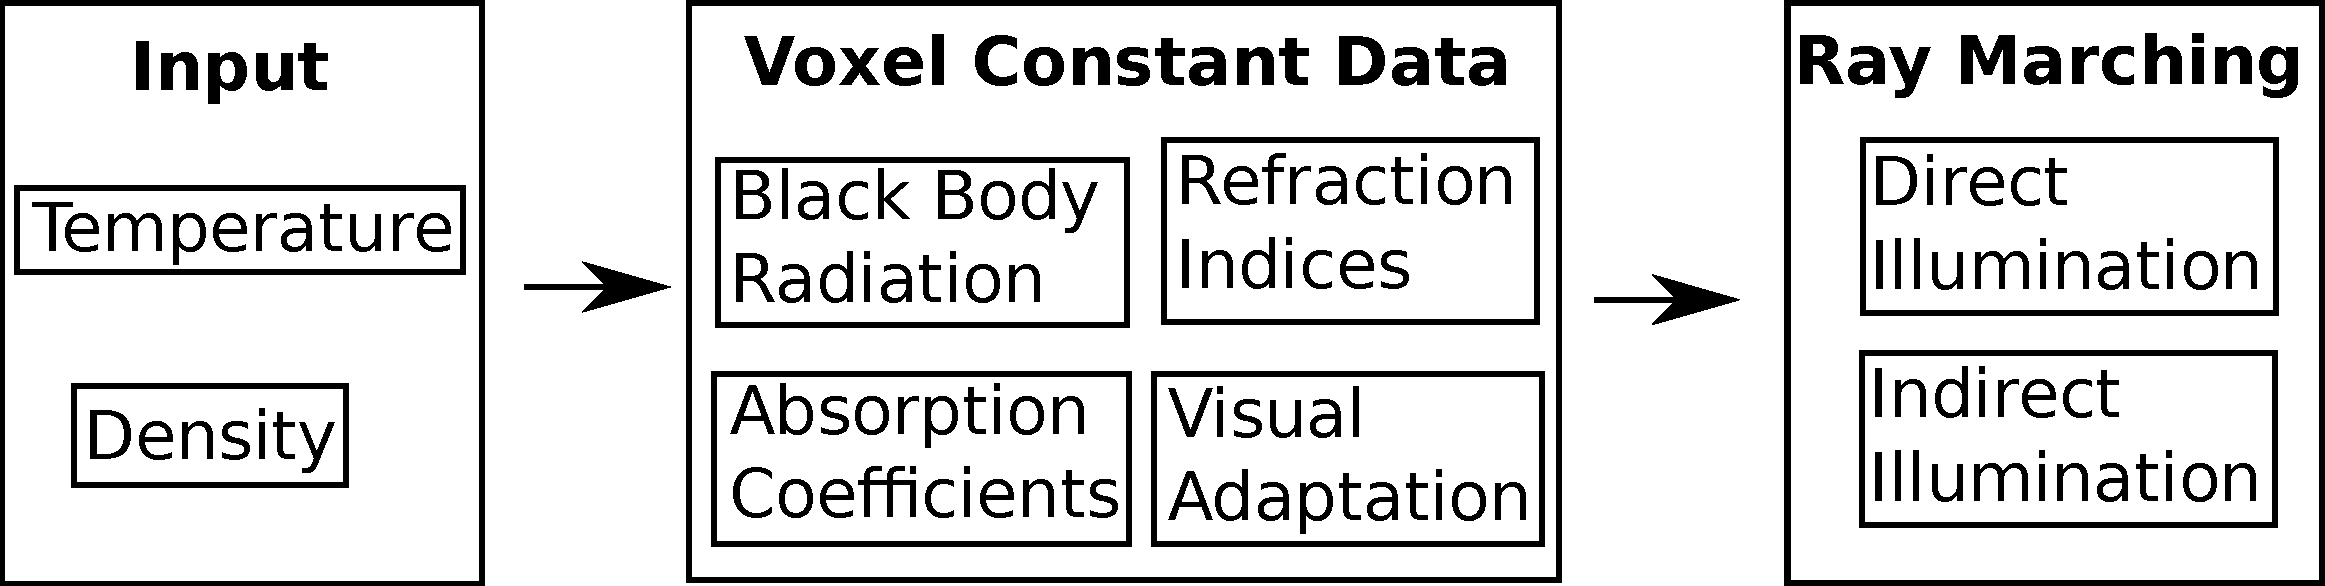
\includegraphics[width=\textwidth]{img/pipeline}
	\caption{An overview of the fire rendering pipeline.}
	\label{fig:pipeline}
\end{figure}

\section{Fundamental Concepts}
\label{sec:fundamental_concepts}

In this section an overview of the fundamentals concepts of volume rendering is presented, readers familiar with the area may proceed to Section~\ref{sec:radiative_transport_equation}.
As the main objective is to give a intuitive introduction into the area, the steps and concepts presented here will not be formally derived.
A simple framework to generate images when light interacts with a participating media will be described. 

The world is modelled as scene were there are a number of elements, the camera, fire volumes, lights and other objects.
The \textbf{camera} is defined as a point and orientation in space, with a projection matrix.
A \textbf{voxel} is defined as a cube in space with some data associated with it.
A \textbf{voxel dataset} is a collection on voxels in space, typically a cubic section of the scene which is divided uniformly into voxels.
There could also be other \textbf{lights sources} in the scene, several types are supported, point, area, directional and cone lights.
\textbf{Other objects} may also be part of the scene, such as polygonal or nurbs meshes.

\begin{figure}[htbp!]
	\centering
	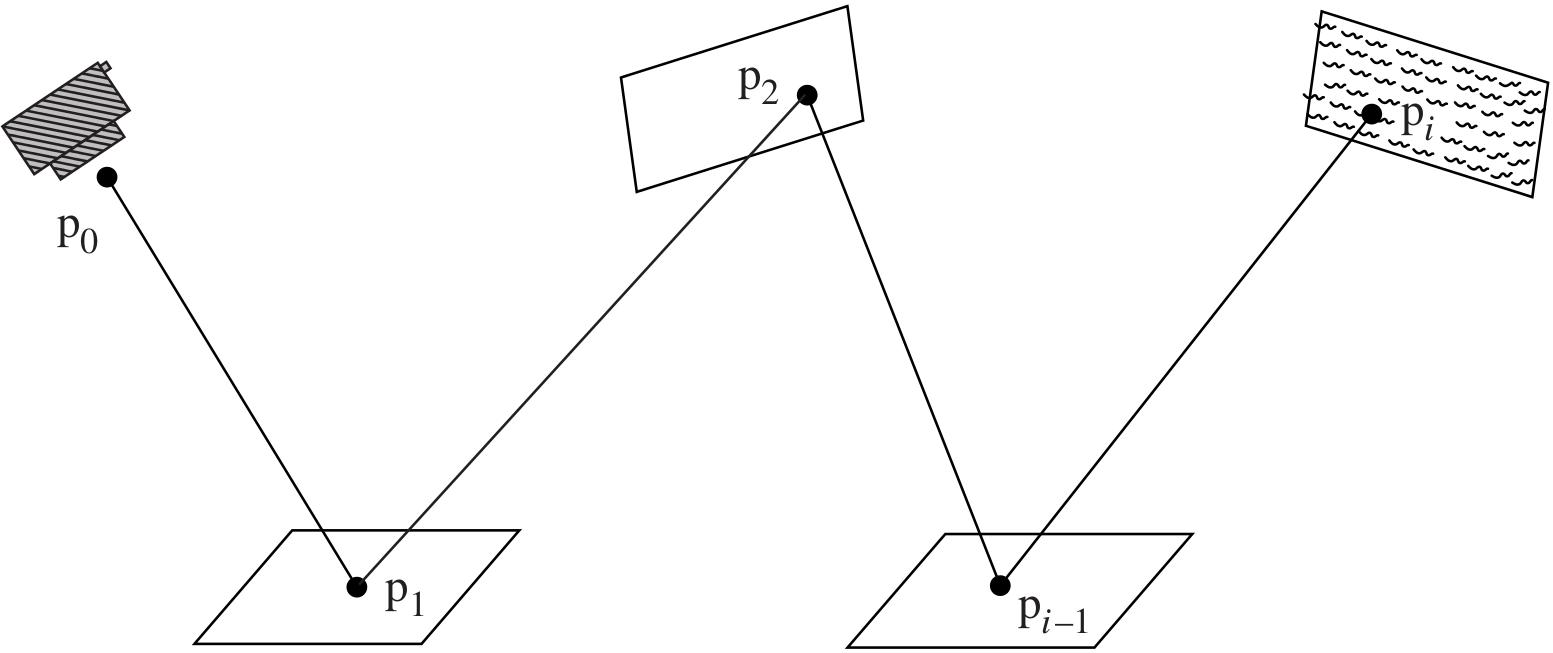
\includegraphics[width=0.6\textwidth]{img/path_tracing}
	\caption{Computing the colour of $p_1$ using path tracing~\cite{Pharr:2010}.}
	\label{fig:path_tracing}
\end{figure}

In order to generate an image from the camera view, path tracing is used to compute the colour of each pixel, as shown in Figure~\ref{fig:path_tracing}.
For each pixel in the camera view, a \textbf{ray} is shot into the scene; whose direction is defined by the camera origin, orientation and the pixel position.
When the ray hits a primitive in the scene, it will be reflected and the colour will depend on the contribution of further intersections along the path.
The final point in the path will be directly connected to a light in the scene, in Figure~\ref{fig:path_tracing}, $p_{i - 1}$ is the final intersection and $p_i$ is the light position.

\section{Radiative Transport Equation}
\label{sec:radiative_transport_equation}

The Radiative Transport Equation (RTE) \cite{Howell:2002} is the model chosen to describe the appearance of any flame in Pegoraro and Parker's method.
The RTE models the variation of spectral radiance $(\omega \nabla) L(\lxo)$ in the medium, where $\lambda$ is a given wavelength in metres, $\x$ is the point of interest in space, and $\omegam$ is a vector that points towards the viewing direction.
Formally, the objective is to get a solution for the RTE for each visible point in the scene, practically, an approximate solution will be computed.

\begin{figure}[htbp!]
	\centering
	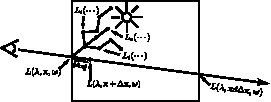
\includegraphics[width=0.9\textwidth]{img/ray_marching_parti}
	\caption{A visual representation of the RTE, where $d$ is the number of $\Delta \x$ between the ray entrance point to the ray exit point.}
	\label{fig:ray_marching_parti}
\end{figure}

The integro-differential Radiative Transport Equation is defined as

\begin{equation}
\begin{split}
(\omega \nabla) L(\lxo) = &- \sigma_a(\lambda, \x) L(\lxo) + \sigma_a(\lambda, \x) L_e(\lxo) \\
&- \sigma_s(\lambda, \x) L(\lxo) + \sigma_s(\lambda, \x) L_i(\lxo),
\end{split}
\end{equation}

where $L_i$ is defined by

\begin{equation}
\label{eq:li}
L_i(\lxo) = \int_{4 \pi} L(\lxo_i) \Phi (\lambda, \omegam, \omegam_i) d \omegam_i,
\end{equation}

where $\sigma_a$ is an absorption coefficient, $\sigma_s$ is a scattering coefficient, $L_e$ is the emitted spectral radiance at the point, $L_i$ is the in-scattering radiance, $\Phi$ is a scattering phase function and $\omega_i$ is a scattering sampling direction.
In order to get an analytical solution to the aforementioned equation, the properties of the medium are assumed to be homogeneous over a small segment $\deltax$ in space,

\begin{equation}
\label{eq:rte_solution_paper}
\begin{split}
L(\lambda, \x + \Delta\x, \omegam) &= e^{-\sigma_t(\lambda, \x) \deltax} L(\lxo) +  \\
& \left(1 - e^{-\sigma_t(\lambda, \x) \deltax} \right) \frac{\sigma_a(\lambda, \x) L_e(\lxo) + \sigma_s(\lambda, \x) L_i(\lxo)}{\sigma_t(\lambda, \x)},
\end{split}
\end{equation}

where $\sigma_t = \sigma_a + \sigma_s$ is the extinction coefficient, a visual depiction of this solution is shown in Figure~\ref{fig:ray_marching_parti}.
To be able to calculate the terms in Equations~\ref{eq:li} and ~\ref{eq:rte_solution_paper}, we will explain in more detail the following factors:

\begin{itemize}
\item Light \textbf{scattering} in the media $L_i(\lxo)$ with a phase function $\Phi(\lambda, \omegam, \omegam_i)$.
\item Emitted light $L_e(\lxo)$ due to \textbf{black body radiation}.
\item Electromagnetic \textbf{absorption}, $\sigma_a$, of certain wavelengths.
\item Due to spatially varying \textbf{refractive} indices, photons may follow non linear paths $\Delta\x$.
\item \textbf{Visual adaptation} processes in the human eye affect the perceived final radiance $L(\lxo)$.
\end{itemize}

\section{Scattering}
\label{sec:scattering}

\begin{figure}[htbp!]
	\centering
	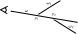
\includegraphics[width=0.5\textwidth]{img/scattering_diag}
	\caption{Photons scattering in the direction of interest.}
	\label{fig:scattering_diag}
\end{figure}

Some photons travelling along arbitrary directions $\omegam_i$, might be scattered in the direction of interest $\omegam$.
A simple diagram of the process is shown in Figure~\ref{fig:scattering_diag}, where two photons travelling in directions $\omegam_1$ and $\omegam_2$, are scattered in the direction of interest $\omegam$, at the points $p_1$ and $p_2$ respectively.
The number of photons which are subjected to this process is controlled by a coefficient $\sigma_s$, the radiance carried by the photons is denoted by $L_i(\lxo)$ and follows a spherical distribution $\Phi (\lambda, \omegam, \omegam_i)$, which was first proposed by~\cite{Henyey:1941} to model diffuse radiation in astronomy,

\begin{equation}
\Phi (\lambda, \omegam, \omegam_i) = \frac{1 - g(\lambda)^2}{4 \pi\left(1 + g(\lambda)^2 - 2 g(\lambda) \omegam \omegam_i\right)^{\frac{3}{2}}},
\end{equation}

where $g$ is an asymmetry coefficient which can be a function of the wavelength, although in most cases it is chosen to be constant.
The value of $g$ must be in the range $(-1, 1)$, where $g < 0$ corresponds to backwards scattering, $g = 0$ to isotropic scattering, and $g > 0$ to forwards scattering.
Monte Carlo techniques can be used to sample the light scattering directions $\omegam_i$.

\section{Black Body Radiation}
\label{sec:black_body_radiation}

\begin{figure}[htbp!]
	\centering
	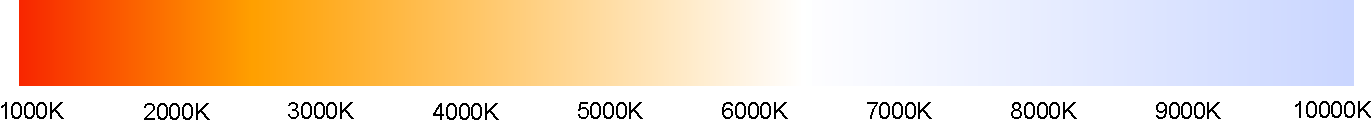
\includegraphics[width=\textwidth]{img/black_body_diag}
	\caption[Cap]{Black body emission colours normalised to ignore brightness\footnotemark.}
	\label{fig:black_body_diag}
\end{figure}

\footnotetext{https://en.wikipedia.org/wiki/File:Blackbody-colours-vertical.svg}
Emitted light from fire, which will illuminate the flame itself and other objects in the scene, is denoted as $L_e(\lxo)$. 
Radiation from an idealized physical body that absorbs all incident electromagnetic radiation can be modelled with Planck's equation for black body radiation, as shown in Figure~\ref{fig:black_body_diag}.
This equation characterizes the electromagnetic radiation $B(T, \lambda, \eta)$ emitted by a black body in thermal equilibrium at a given temperature $T$.

\begin{equation}
L_e(\lxo) = B(T, \lambda, \eta) = \frac{2 h c^2}{\lambda^5  (e ^\frac{h c}{\lambda k T} - 1)},
\end{equation}

where $h = 6.62606957 \times 10^{-34}~J/s$ is Planck's constant, $k = 1.3806488 \times 10^{-23}~J/K$ is Boltzmann constant, $\eta$ is the refraction index of the medium and $c =  c_0 / \eta$ is the speed of light in the current medium, where $c_0 = 299792458~m/s$ is the speed of light in a vacuum. 
The refraction index $\eta$ varies across the medium, the procedure to compute it will be described in Section~\ref{sec:refraction}.

\section{Absorption coefficients}
\label{sec:absorption_coefficients}

As fire is not an idealized black body radiator, certain wavelengths are not present in the emitted radiance.
This behaviour can be modelled using absorption coefficients for each chemical that would mask the undesired wavelengths, such that

\begin{equation}
\sigma_a L_e(\lxo) = \sum_{i = 0}^N \sigma_{ai} B_i(T, \lambda, \eta),
\end{equation}

where $N$ is the number of different chemical species in the mix, $\sigma_{ai}$ and $B_i(T, \lambda, \eta)$ are the absorption coefficient and light emission of the $i^{th}$ chemical.
In the interest of simplicity, the absorption and radiation effects for \textbf{soot} will be treated separately from those caused by other \textbf{chemical species}.

\subsection{Soot Absorption}
\label{sec:soot_absorption}

Light generated by incandescent soot accounts for most of the total radiance emitted by a flame. 
The spectral absorption coefficient of soot is defined as

\begin{equation}
\sigma_a(\lambda, \x) = \frac{48 N(\x) \pi R^3 n m}{\lambda^{\alpha(\lambda)} ((n^2 - m^2 +2)^2 + 4 n^2 m^2)},
\end{equation}

where $N(\x)$ is the number density, density per unit volume, $R$ is the radius of a soot particle, $n$, $m$ and $\alpha(\lambda) = 1.39$ are optical constants for different types of soot.
In Table~\ref{tb:soot_absorption_coefficients}, values for the optical constants $n$ and $m$ are provided for several materials, the data was obtained from~\cite{Dalzell:1969}.
The radius of soot particles was determined in the range $R \in \lbrace 50\mbox{~\AA} \ldots 800\mbox{~\AA} \rbrace $ by~\cite{Dalzell:1969}.
Since our data is defined with soot densities, we have chosen the radius to be the mean value $R = 425 \times 10^{-10}$ metres.

\begin{table}[htbp!]
\centering
\caption{Absorption constants for propane and acetylene, wavelengths are in nanometres.}
\label{tb:soot_absorption_coefficients}
\begin{tabular}{cc|c|c|c|c|}
\cline{3-6}
                                                 &    & \multicolumn{4}{c|}{\textbf{Wavelengths}} \\ \cline{3-6} 
                                                 &    & 435.8   & 450    & 550   & 650   \\ \hhline{--|=|=|=|=|}
\multicolumn{1}{|c|}{\multirow{2}{*}{\textbf{Propane}}}   & \multicolumn{1}{c||}{n}  & 1.57    & 1.56   & 1.57  & 1.56  \\ \cline{2-6} 
\multicolumn{1}{|c|}{}                           & \multicolumn{1}{c||}{nm} & 0.46    & 0.5    & 0.53  & 0.52  \\ \hline
\multicolumn{1}{|c|}{\multirow{2}{*}{\textbf{Acetylene}}} & \multicolumn{1}{c||}{n}  & 1.56    & 1.56   & 1.56  & 1.57  \\ \cline{2-6} 
\multicolumn{1}{|c|}{}                           & \multicolumn{1}{c||}{nm} & 0.46    & 0.48   & 0.46  & 0.44  \\ \hline
\end{tabular}
\end{table}

\FloatBarrier
\subsection{Absorption From Other Chemical Species}
\label{sec:absorption_from_chemical_species}

Flames of more uncommon colours are generally produced when using salts of different chemicals.
The spectral line emitted by an particular atom depends of the electronic transitions between different energy levels.
The absorption coefficients associated for a given spectral frequency and a known atomic element can be computed as


\begin{equation}
\sigma_a(\lambda, \x) = \frac{\phi(\lambda) N_2 A_{21} \lambda^4 (e ^\frac{h c}{\lambda k T} - 1)}{8 \pi c}
\end{equation}

where $\phi(\lambda)$ is the normalized spectral line, $N_2$ is the number density (number of particles per unit volume), $A_{21}$ is an Einstein coefficient measuring the transition probabilities of spontaneous emission.

\section{Refraction}
\label{sec:refraction}

Heat emanating from the flame is transferred to the air which surrounds it.
Since the refractive index of a medium depends on its temperature, light transiting the space near the flame will follow non linear paths due to varying refractive indices.
Fresnel equations describe in detail both reflection and refraction effects, as shown in Figure~\ref{fig:refraction_diag}, when a wave moves between media with different refractive indices.
Schlick equations~\cite{Schlick1994} are widely used by the computer graphics community to approximate the Fresnel coefficients.

\begin{figure}[htbp!]
	\centering
	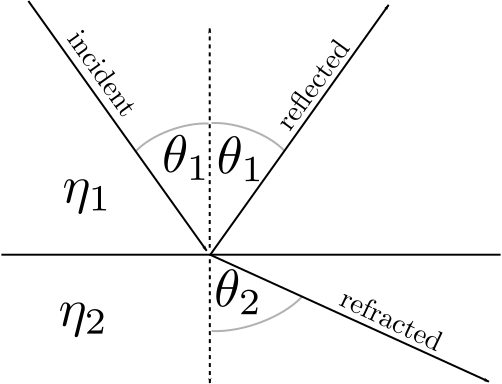
\includegraphics[width=0.4\textwidth]{img/refraction_diag}
	\caption{Ray being refracted and reflected in the boundary between two media.}
	\label{fig:refraction_diag}
\end{figure}

The fraction of light which is reflected is assumed to be negligible for combustion phenomena; thus, the refraction angles for the rays can be easily computed using Snell's law

\begin{equation}
\frac{\sin \theta_1}{\sin \theta_2} = \frac{\eta_2}{\eta_1},
\end{equation}

where $\theta_1$ is the incident angle, $\theta_2$ is the refracted angle, $\eta_1$ is the index of refraction of the media which the ray is coming from and $\eta_2$ is the index of refraction of the media which the ray is going to.
The values for all the constants in this section are defined in Table~\ref{tb:ciddor_constants}.

\cite{Ciddor:1996} proposed a method to compute the refractive indices of air 

\begin{equation}
\label{eq:ciddor_eta_air}
\eta_{air} = 1 + \frac{\rho_a \eta_{axs}}{\rho_{axs}} + \frac{\rho_w \eta_{ws}}{\rho_{ws}},
\end{equation}

where $\rho_{axs}$ is the density of dry air, $\rho_{ws}$ is the density of pure water vapour, $\rho_{a}$ and $\rho_{w}$ are the equivalent quantities for dry air, $\eta_{axs}$ is the refractive index for $CO_2$ and $\eta_{ws}$ is the refractive index for water vapour.
The refractive index for $CO_2$ is estimated as

\begin{align}
\label{eq:ciddor_eta_axs}
\eta_{axs} &= \eta_{as} \left(1 + 0.534 \times 10^{-6} \left(x_c - 450 \right) \right), \\
\label{eq:ciddor_eta_as}
\eta_{as} &= 10^{-8} \left( \frac{k_1}{k_0 - \lambda} + \frac{k_3}{k_2 - \lambda} \right),
\end{align}

where $x_c \in \lbrace 300 \ldots 450 \rbrace $ is the proportion in parts per million of $CO_2$, $k_0$, $k_1$ $k_2$ and $k_3$ are constants, and $\lambda$ is the wave number (reciprocal of the vacuum wavelength).
The refractive index for water vapour is computed as

\begin{equation}
\label{eq:ciddor_eta_ws}
\eta_{ws} = 1.022 \times 10^{-8} \left( w_0 + w_1 \lambda + w_1 \lambda^2 + w_3 \lambda^3 \right),
\end{equation}

where $w_0$, $w_1$, $w_2$ and $w_3$ are constants.

The $\rho$ densities are computed as follows

\begin{equation}
\label{eq:ciddor_rho}
\rho =  \frac{p m_a}{zrT} \left( 1 - x_w \left(1 - \frac{m_w}{m_a} \right) \right), 
\end{equation}

where $p$ is the pressure in pascals, $r$ and $m_w$ are constants, 

\begin{align}
\label{eq:ciddor_m_a}
m_a &= 0.0289635 + 12.011 \times 10^{-8}(x_c - 400)),\\
\label{eq:ciddor_z}
z &= 1 - \frac{p}{T} \left(a_0 + a_1 t + a_2 t^2 + \left(b_0 + b_1 t \right) x_w + \left(c_0 + c_1 t \right) x_w^2 \right) + \left( \frac{p}{T} \right)^2 \left( d + ex_w^2 \right),
\end{align}

where $a_0$,  $a_1$, $a_2$,  $b_0$,  $b_1$,  $c_0$,  $c_1$,  $d$ and $e$ are constants.

\begin{align}
\label{eq:ciddor_t}
T &= t + 273.15, \\
\label{eq:ciddor_x_w}
x_w &= \frac{f h v}{ p}, \\
\label{eq:ciddor_f}
f &= \alpha + \beta p + \gamma t^2,
\end{align}

where $\alpha$, $\beta$ and $\gamma$ are constants, and $h \in \lbrace 0 \ldots 1 \rbrace$ is the air relative fractional humidity, $0$ for dry air and given by the user for moist air.

The pressure $p$ can also be computed using the ideal gas law
\begin{equation}
\label{eq:ciddor_p}
pV=\frac{NRT}{V} = n T,
\end{equation}

where $N$ is the number of molecules, $V$ is the total volume of the gas, $T$ is the temperature of the gas, $n$ is the number density (number of particles per unit volume), $R = k N_a$, where $k$ is the Boltzmann constant and $N_a$ is Avogadro constant.

Depending on the situation, there are two acceptable methods to compute the vapour pressure $v$, both are described below.

\subsection{Davis' Saturation Vapour Pressure}
\label{subsec:davis_v}

In \cite{Ciddor:1996} paper, the author used the method proposed by~\cite{Davis:1992} to compute the saturation of vapour pressure

\begin{equation}
\label{eq:davis_v}
v = e^{AT^2 + BT + C + D/T},
\end{equation}

where $A$, $B$, $C$ and $D$ are constants.
This equation is relatively easy to compute, however incorrect results will be obtained for temperatures below $0\C$.
As we are concerned with fire rendering, which entails high temperatures, this method is preferred due to its simplicity.

\subsection{Huang's Saturation Vapour Pressure}
\label{subsec:huang_v}

The International Association for the Properties of Water and Steam (IAPWS) adopted an alternative technique to~\cite{Davis:1992}, which was proposed by~\cite{Huang:1998}.
The more recent method addresses the drawbacks of the previous technique, giving reasonable results for temperatures below $0\C$.
Nevertheless, the generality comes with increased complexity in the equations

\begin{align}
\label{eq:huang_v}
v &= 10^{6} \left( \frac{2C}{X} \right)^4, \\
X &= -B + \left( B^2 - 4AC \right)^{\frac{1}{2}}, \\
\begin{bmatrix}
A \\
B \\
C
\end{bmatrix} &=
\begin{bmatrix}
1 & K_1 & K_2 \\
K_3 & K_4 & K_5 \\
K_6 & K_7 & K_8 \\
\end{bmatrix} 
\begin{bmatrix}
~\Omega^2 \\
\Omega \\
1
\end{bmatrix}, \\
\Omega &= T + \frac{K_9}{T - K_{10}},
\end{align}

where $K_1$, $K_2$, $K_3$, $K_4$, $K_5$, $K_6$, $K_7$, $K_8$, $K_9$, and $K_{10}$ are constants.

\subsection{Ciddor's Method Summary}

The inputs of Ciddor's technique are a wavelength $\lambda_0$, a temperature $t$, a pressure $p$, a relative humidity value $h$ and a $CO_2$ concentration $x_c$.
The values for all the constants needed for the method are defined in Table~\ref{tb:ciddor_constants}.
A refraction index is computed following this method for each voxel in the volumetric data structure.
The steps to compute the index of refraction are listed below

\begin{enumerate}
\item Let $z_a = 0.9995922115$, computed using Equation~\ref{eq:ciddor_z} with $t = 20~\C$, $p = 101.325~Pa$ and $x_w=0$.
\item Calculate $\lambda = 1 / \lambda_0^2$, and $T$ with Equation~\ref{eq:ciddor_t}.
\item Calculate $v$ with the method described in Section~\ref{subsec:davis_v} or in Section~\ref{subsec:huang_v}.
\item Calculate $x_w$ using Equations~\ref{eq:ciddor_f} and~\ref{eq:ciddor_x_w}.
\item Calculate $\eta_{as}$ using Equation~\ref{eq:ciddor_eta_as}.
\item Calculate $\eta_{ws}$ using Equation~\ref{eq:ciddor_eta_ws}.
\item Calculate $m_a$ using Equation~\ref{eq:ciddor_m_a}.
\item Calculate $\eta_{axs}$ using Equation~\ref{eq:ciddor_eta_axs}.
\item Calculate $z_m$ using Equation~\ref{eq:ciddor_z}.
\item Calculate $\rho_{axs} = (p_0 m_a)/(z_a r T_0)$, where $p_0 = 101325$, and $T_0 = 288.15$, using Equation~\ref{eq:ciddor_rho}.
\item Calculate $\rho_{w} = (x_w p m_w)/(z_m r T)$ using Equation~\ref{eq:ciddor_rho}.
\item Calculate $\rho_{a} = ((1 - x_w) p m_a)/(z_m r T)$ using Equation~\ref{eq:ciddor_rho}.
\item Calculate the index of refraction $\eta_{air}$ using Equation~\ref{eq:ciddor_eta_air}.
\end{enumerate}

\renewcommand{\arraystretch}{1.2} % Add extra vertical space, otherwise the equations look awful in the table
\begin{table}[htbp!]
\centering
\caption{Values for the constants in the equations used to compute the index of refraction.}
\label{tb:ciddor_constants}
\begin{tabular}{|l|l|l|l|l|}
\cline{1-2} \cline{4-5}
\textbf{Name}        & \textbf{Value}                       &  & \textbf{Name}     & \textbf{Value}                                \\ \cline{1-2} \cline{4-5} 
$\rho_{ws}$ & 0.00985938                  &  & $a_0$    & $1.58123~\times 10 ^{-6} K Pa^{-1}$  \\ \cline{1-2} \cline{4-5} 
$x_c$       & $450~ppm$                   &  & $a_1$    & $-2.9331 ~\times 10 ^{-8} Pa^{-1}$   \\ \cline{1-2} \cline{4-5} 
$k_0$       & $238.0185~\mu m^{-2}$       &  & $a_2$    & $1.1043 ~\times 10 ^{-10} Pa^{-1}$   \\ \cline{1-2} \cline{4-5} 
$k_1$       & $5792105~\mu m^{-2}$        &  & $b_0$    & $5.707~\times 10 ^{-6} K Pa^{-1}$    \\ \cline{1-2} \cline{4-5} 
$k_2$       & $57.362~\mu m^{-2}$         &  & $b_1$    & $-2.051~\times 10 ^{-8} Pa^{-1}$     \\ \cline{1-2} \cline{4-5} 
$k_3$       & $167917~\mu m^{-2}$         &  & $c_0$    & $1.9898~\times 10 ^{-4} K Pa^{-1}$   \\ \cline{1-2} \cline{4-5} 
$w_0$       & $295.235~\mu m^{-2}$        &  & $c_1$    & $-2.376~\times 10 ^{-6} K Pa^{-1}$   \\ \cline{1-2} \cline{4-5} 
$w_1$       & $2.6422~\mu m^{-2}$         &  & $d$      & $1.83~\times 10 ^{-11} K^2 Pa^{-2}$  \\ \cline{1-2} \cline{4-5} 
$w_2$       & $-0.03238~\mu m^{-2}$       &  & $e$      & $-0.765~\times 10 ^{-8} K^2 Pa^{-2}$ \\ \cline{1-2} \cline{4-5} 
$w_3$       & $0.004028~\mu m^{-2}$       &  & $\alpha$ & $1.00062$                            \\ \cline{1-2} \cline{4-5} 
$p$         & $1~atm~ = 101 325~Pa$       &  & $\beta$  & $3.14 \times 10^{-8} Pa^{-1}$        \\ \cline{1-2} \cline{4-5} 
$r$         & $8.31451~J mol^{-1} K^{-1}$ &  & $\gamma$ & $5.6 \times 10^{-7} \C^{-2}$         \\ \cline{1-2} \cline{4-5} 
$m_w$       & $0.018015~kg/mol$           &  & $k$      & $1.3806488 \times 10^{-23}~J/K$      \\ \cline{1-2} \cline{4-5} 
$N_a$ & $6.02214129 \times 10^{23}~mol^{-1}$ &  & $K_4$  & $1.20208247025 \times 10^{4}$   \\ \cline{1-2} \cline{4-5} 
$A$   & $1.2378847 \times 10^{-5} K^{-2}$    &  & $K_5$  & $-3.23255503223 \times 10^{6}$  \\ \cline{1-2} \cline{4-5} 
$B$   & $-1.9121316 \times 10^{-2} K^{-1}$   &  & $K_6$  & $1.49151086135 \times 10$       \\ \cline{1-2} \cline{4-5} 
$C$   & $33.93711047$                        &  & $K_7$  & $-4.82326573616 \times 10^{3}$  \\ \cline{1-2} \cline{4-5} 
$D$   & $-6.3431645 \times 10^3 K$           &  & $K_8$  & $4.05113405421 \times 10^{5}$   \\ \cline{1-2} \cline{4-5} 
$K_1$ & $1.16705214528 \times 10^{3}$        &  & $K_9$  & $-2.38555575678 \times 10^{-1}$ \\ \cline{1-2} \cline{4-5} 
$K_2$ & $-7.24213167032 \times 10^{5}$       &  & $K_{10}$ & $6.50175348448 \times 10^{2}$   \\ \cline{1-2} \cline{4-5} 
$K_3$ & $-1.70738469401 \times 10$           &  &        &                                 \\ \cline{1-2} \cline{4-5}
\end{tabular}
\end{table}
\renewcommand{\arraystretch}{1} % Restore to previous value

\FloatBarrier
\section{Visual Adaptation}
\label{sec:visual_adaptation}

The human eye presents a non-linear response to incident radiance $L$, as shown in Figure~\ref{fig:pegoraro_2006_adaptation}.
If a flame is the dominant light source in a scene, it will appear with yellow-white colours, while the same flame in an environment with comparable or brighter lights might appear orange-yellow.

\begin{figure}[htbp!]
	\centering
	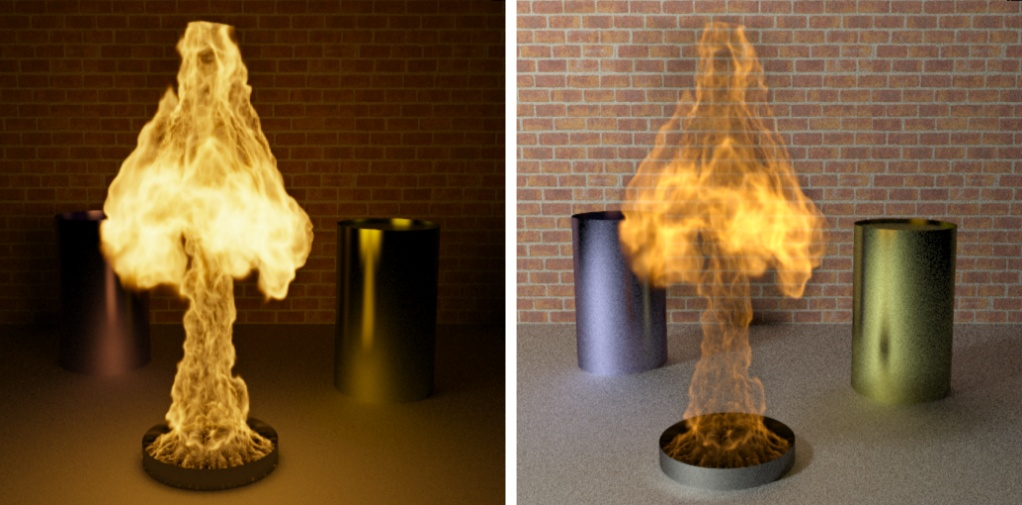
\includegraphics[width=0.6\textwidth]{img/pegoraro_2006_adaptation}
	\caption{Fire variations in colour due to eye adaptation mechanisms~\cite{Pegoraro:2006}.}
	\label{fig:pegoraro_2006_adaptation}
\end{figure}

A simple equation which can model this phenomena was proposed by~\cite{Naka:1966}

\begin{equation}
\label{eq:visual_adaptation}
R(L, \tau) = \frac{L}{L + \tau},
\end{equation}

where $\tau$ is a non-linear adaptation state.
This state is determined by the visual system to maximize the perception of features for a given scene.
Several approaches have been proposed to determine which features are used and how to compute the optimal state.
We refer the readers to~\cite{Fairchild:2005} for an in depth review of visual adaptation methods.
The Von Kries model~\cite{Fairchild:2005}, the new values for the LMS cone responses for a given stimulus are simply multiplied by the inverse of the maximum response in the scene.
The Retinex model~\cite{Fairchild:2005}, extends Von Kries' work by normalizing the the ratio of the stimulus with the average response in a retinex space.
The retinex space is defined as a three dimensional space with the spectral responses of the cones.
\cite{Irawan:2005} presented neural network-based model which includes time varying adaptations, and variations due to intrinsic observer characteristics, such as their age or visual impairment, are also considered.


%------------------------------------------------------------------------------
\chapter{Implementation details}
\label{ch:implementation_details}

In this chapter we will explain how to use the shaders which have been implemented and the minor differences between the theoretical pipeline explained in Chapter~\ref{ch:methodology} and the actual software implementation.
An overview of the pipeline is shown in Figure~\ref{fig:pipeline_simplified}, note that modules in grey have not been implemented.

\begin{figure}[htbp!]
	\centering
	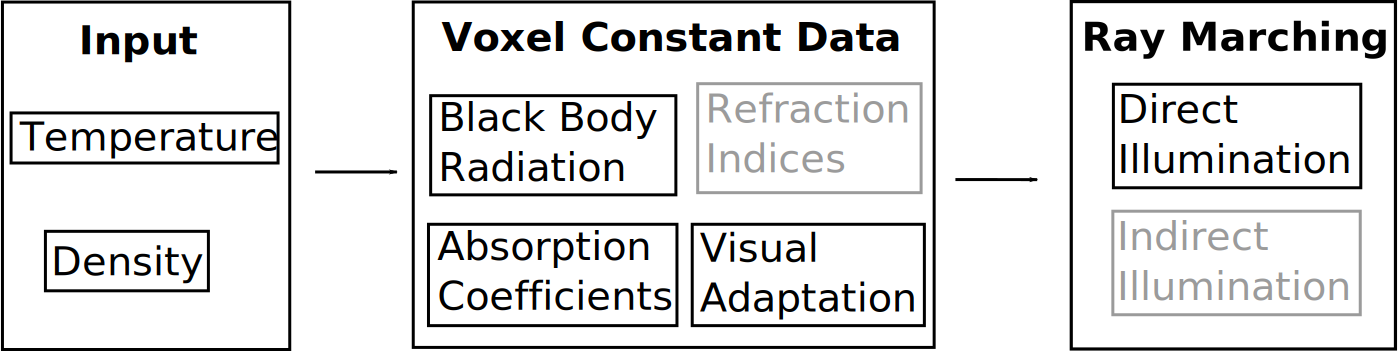
\includegraphics[width=\textwidth]{img/pipeline_simplified}
	\caption{An overview of the implemented fire rendering pipeline.}
	\label{fig:pipeline_simplified}
\end{figure}

\section{Application Overview}
\label{sec:application_overview}

The model chosen for our data is that of a three-dimensional voxel dataset, a cube in space is uniformly divided and a data value is stored for each voxel.
This data is either a soot density estimate for the \textit{fire volume shader} or a temperature estimate for the \textit{fire light shader}.
Three file formats are supported, dense and sparse float voxel data is ASCII, and sparse binary RGBA values, as shown in Figure~\ref{fig:file_format}.
In the ASCII dense format, the file first line are three integers, separated by spaces, declaring the width, height and depth of the data, followed by $w \cdot h \cdot d$ lines with a single floating point values.
The ASCII sparse format, has two extra parameters in the first line, $c$ is the number of data points in the file and $b$ is the default value for any voxel that is not specified in the file.
Each data line has the $x,y,z$ coordinates and the data values are separated by spaces.
The binary sparse format starts with a 4 byte integer declaring how many data points are in the file, each voxel has its coordinates $x,y,z$ as 4 bytes integers and a rgb alpha colour, where each channel is an 8 bytes floating point double value.
Values not included in the file are considered to be initialized to zero. 

\begin{figure}[htpb!]
        \centering
        \begin{subfigure}[t]{0.2\textwidth}
                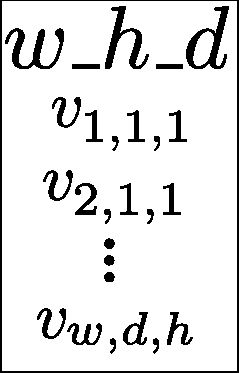
\includegraphics[width=\textwidth]{img/file_format_ascii_dense}
                \caption{ASCII dense (*.vol).}
                \label{fig:file_format_ascii_dense}
        \end{subfigure}%
        ~ %add desired spacing between images, e. g. ~, \quad, \qquad, \hfill etc.
          %(or a blank line to force the subfigure onto a new line)
        \begin{subfigure}[t]{0.3\textwidth}
                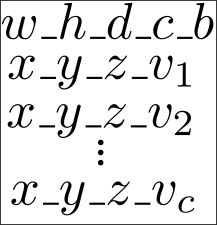
\includegraphics[width=\textwidth]{img/file_format_ascii_sparse}
                \caption{ASCII sparse (*.uintah).}
                \label{fig:file_format_ascii_sparse}
        \end{subfigure}
        ~ %add desired spacing between images, e. g. ~, \quad, \qquad, \hfill etc.
          %(or a blank line to force the subfigure onto a new line)
        \begin{subfigure}[t]{0.282\textwidth}
                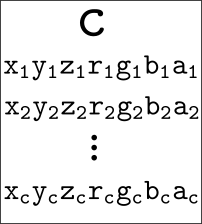
\includegraphics[width=\textwidth]{img/file_format_binary}
                \caption{Binary sparse (*.raw).}
                \label{fig:file_format_binary}
        \end{subfigure}
        \caption{Suported file formats, $\_$ represent the character space.}
        \label{fig:file_format}
\end{figure}

\section{\MentalRay Rendering Approach}
\label{sec:mental_ray_rendering_approach}

How mental ray shoots rays around and what is its paradigm.

\MentalRay approach to solving the rendering equation is based on path tracing, as shown in Figure~\ref{fig:mental_ray_model}, for each pixel in the camera view, an eye ray will be shot in the scene.
On an intersection with an object in the scene, its material shader will be called, this shader will shoot a light ray for each light in the scene, which in effects calls the light shader of the given light.
In order to compute the irradiance at the intersection point, the light shader will probably trace a shadow ray from the light to the intersection point.
Eventually, the material shader will compute the final colour with the information received from the light shader. 

\begin{figure}[htbp!]
\centering
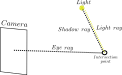
\includegraphics[width=0.8\textwidth]{img/mental_ray_model}
	\caption{\MentalRay simple ray casting example.}
	\label{fig:mental_ray_model}
\end{figure}

Under this assumptions, the steps required to solve the RTE, Equation~\ref{eq:rte_solution_paper}, are:

\begin{enumerate}
\item Shoot a ray from the eye into the scene.
\item If the ray intersects the fire volume, perform ray marching in the volume.
	\begin{enumerate}
	\item Compute direct illumination at the current point.
		\begin{enumerate}
		\item Get initial radiance using black body radiation.
		\item Attenuate with absorption coefficient.
		\end{enumerate}	
	{\color{gray} \item Compute indirect illumination at the current point.
		\begin{enumerate}
		\item Use phase function to get the scattered light distribution.
		\end{enumerate}}
	\item Advance to next point in ray marching.
		\begin{enumerate}
		{\color{gray} \item Change ray direction using refraction index.}
		\end{enumerate}	
	\end{enumerate}
\item Compute eye visual adaptation to fire colour.
\end{enumerate}

\section{Simplifications}
\label{sec:simplifications}

Equation~\ref{eq:rte_solution_paper} provides a radiance value, $L(\lambda, \x + \Delta\x, \omegam)$ for the next march increment, however it is more intuitive to think about the final radiance $L(\lambda, \x, \omegam)$, for the first intersection point.
The radiance at the interest point is given by 

\begin{equation}
\begin{split}
L(\lambda, \x, \omegam) &= e^{-\sigma_t(\lambda, \x) \deltax} L(\lambda, \x + \Delta\x, \omegam) +  \\
& \left(1 - e^{-\sigma_t(\lambda, \x) \deltax} \right) \frac{\sigma_a(\lambda, \x) L_e(\lxo) + \sigma_s(\lambda, \x) L_i(\lxo)}{\sigma_t(\lambda, \x)}.
\end{split}
\end{equation}

In fire phenomena the effect of scattered light in the final image is practically imperceptible~\cite{Pegoraro:2006}.
Intuitively, it means that as the medium is highly emissive and thin, most of the emitted photons have their initial paths unaltered.
The scattering directions $\omegam_i$ are in essence sampling directions over a sphere of scattered light $L_i$.
In practice, the simplification will significantly decrease rendering time, as $\omegam_i$ would have to be sampled by means of a computationally expensive Monte Carlo approximation. 
Exploiting the previous prior knowledge, the scattering contributions can be safely ignored by setting $\sigma_s = 0$, which simplifies the previous equation to

\begin{equation}
L(\lambda, \x, \omegam) = e^{-\sigma_a(\lambda, \x) \deltax} L(\lambda, x + \Delta\x, \omegam) +  \left(1 - e^{-\sigma_a(\lambda, \x) \deltax} \right) L_e(\lxo).
\end{equation}

A visual representation of the implications of the aforementioned simplification is shown in Figure~\ref{fig:ray_marching}.
Note that a single point light is used in the diagram to avoid clutter, yet in our implementation there is a point light located at the centre of each voxel whose temperature is high enough to be emissive.
The non-linear trajectories of the photons, of the rays in practice, due to varying refraction indices in the media were also outside of the scope of this project.
Deformations produced by the refraction phenomena can be noticeable, however there are important simplifications in the implementation if we choose to ignore them.
Namely, we can reduce the recursiveness significantly, instead of starting in the first intersection and recursively solve the equation, we can start from the end point and accumulate the result backwards with a loop, as computing the end point is this situation is trivial.

\begin{figure}[htbp!]
	\centering
	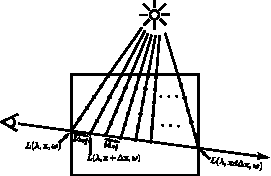
\includegraphics[width=0.8\textwidth]{img/ray_marching}
	\caption{Calculating the illumination values for samples along a ray.}
	\label{fig:ray_marching}
\end{figure}

\section{Shaders}
\label{sec:shaders}

Talk about things like which parts are written in parallel code, instance support, shader internal memory, sparse data, how the software escalates, memory consumption, Maya integration, spectrum to RGB integration, maybe more details about units for black body radiation and everything that was not explained before.

In order to be able to implement the different parts of our architecture, input data, voxel constant data, etc, without a monolithic design, lead to shader organization depicted in Figure~\ref{fig:shaders_diagram}.
The temperature and density shaders will read the raw input values, the emission and absorption shaders will compute respectively, black body radiation and absorption coefficients.
The fire light shader will sample and compute emitted light $L_e$, and the fire volume shader is in charge of adding absorption from light to interest point and to perform the main ray marching computations. 

\begin{figure}[htbp!]
	\centering
	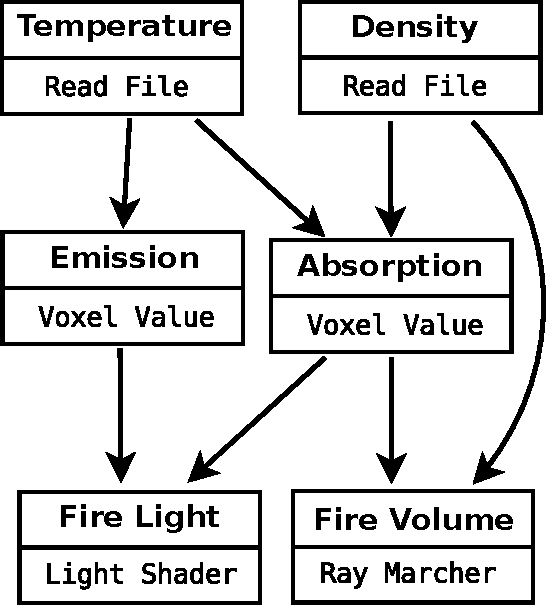
\includegraphics[width=0.4\textwidth]{img/shaders_diagram}
	\caption{Diagram depicting the shaders and their interconnections.}
	\label{fig:shaders_diagram}
\end{figure}

\begin{figure}[htpb!]
        \centering
        \begin{subfigure}[b]{0.7\textwidth}
                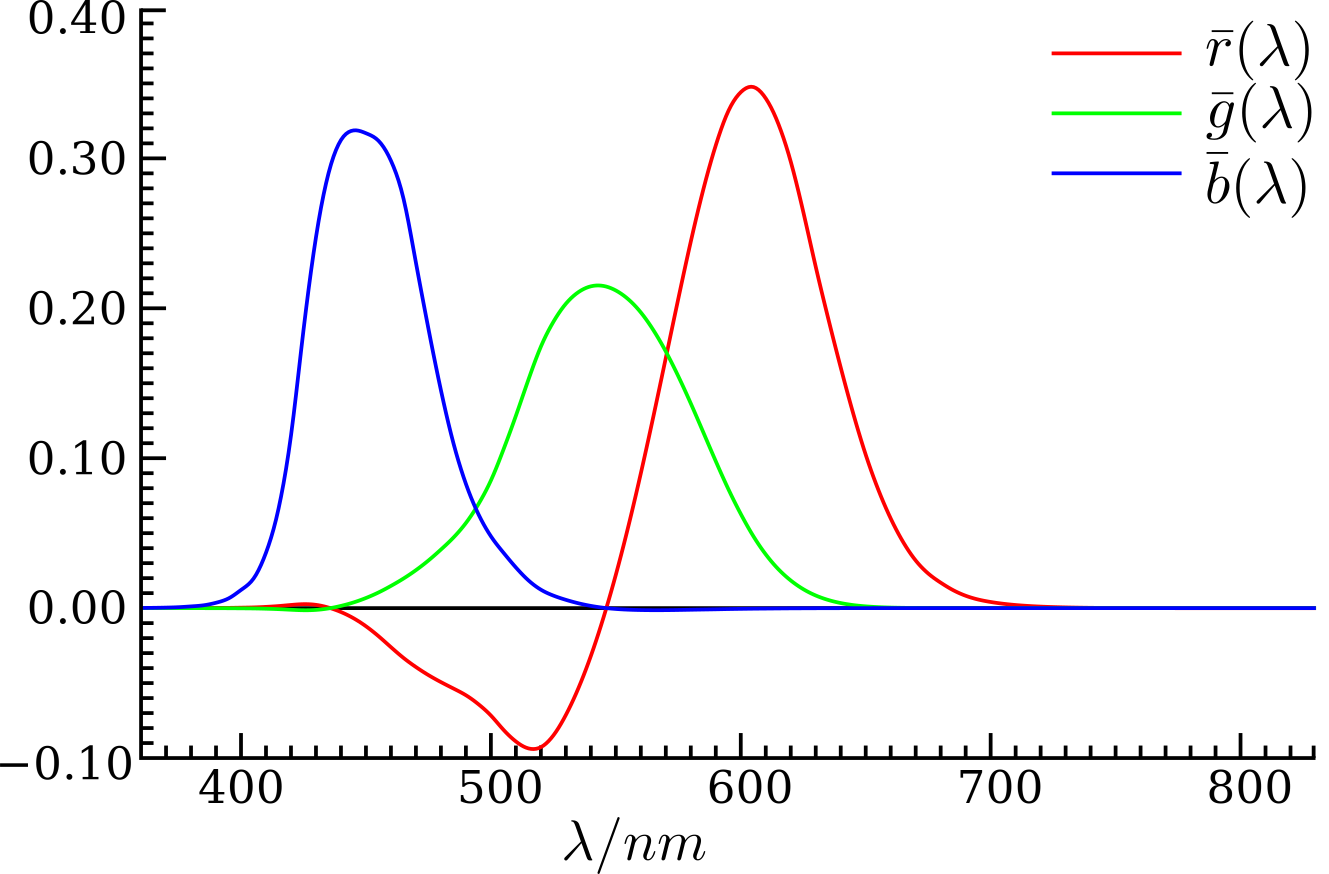
\includegraphics[width=\textwidth]{img/CIE_RGB}
                \caption{Spectral tristimulus values for CIE RGB~\cite{CIE_RGB}.}
                \label{fig:cie_rgb}
        \end{subfigure}%
        \quad %add desired spacing between images, e. g. ~, \quad, \qquad, \hfill etc.
          %(or a blank line to force the subfigure onto a new line)
        \begin{subfigure}[b]{0.7\textwidth}
                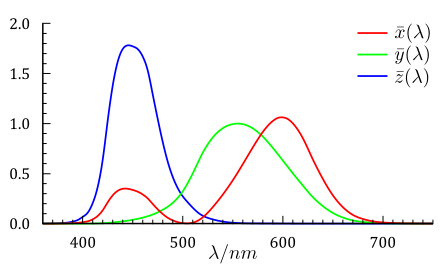
\includegraphics[width=\textwidth]{img/CIE_XYZ}
                \caption{Spectral tristimulus values for CIE XYZ~\cite{CIE_XYZ}.}
                \label{fig:cie_xyz}
        \end{subfigure}
        \caption{Colour matching curves for RGB and XYZ spaces.}
\end{figure}

Volumetric data tends to be quite sparse, and usually we are working with volumes of $256 \times 256 \times 256$, which assuming a standard 32 bits floating point value per voxel, accumulates to 64 megabytes of data.
With the shader architecture shown in Figure~\ref{fig:shaders_diagram}, there will be at least four copies of those structures per fire in the scene.
A total of 256 megabytes per voxel dataset is unacceptable, we dealt with the problem using an open source sparse voxel dataset library~\cite{OpenVDB}.

To speed up the render time, all spectrum related computations are integrated at source to RGB coefficients.
Our spectrum class has a number of samples that can be set at compile time, 30 samples were used in all of our renderings.
To compute the absorption coefficients that were introduced in Section~\ref{sec:absorption_coefficients}, data from Table~\ref{tb:soot_absorption_coefficients} is used.
As there is not enough data to compute the 30 spectrum coefficients, a linear interpolation is used to fill the missing values.
RGB coefficients are the standard colour representation in computer screens, however not every colour visible by the human eye can be reproduced in RGB space.
There are further disadvantages inherent to this representation, for example certain colours visible by the human eye would require negative values for the $\bar{r}(\lambda)$ coefficient, as shown in Figure~\ref{fig:cie_rgb}.
The XYZ colour space is built using three sets of imaginary primaries, which have a series of favourable properties.
Any colour which can be seen by the human eye can be represented with some $x(\lambda)$, $y(\lambda)$, $z(\lambda)$ coefficients, the Y channel is equal to the photopic luminous efficiency function $V(\lambda)$, which models the variation of perceived brightness, and as shown in Figure~\ref{fig:cie_xyz}, the coefficients are always positive.

Given a Spectral Power Distribution (SPD) $S(\lambda)$, the $x$, $y$, $z$ coefficients for $S(\lambda)$ in the XYZ space are defined with respect to spectral matching curves $X(\lambda)$, $Y(\lambda)$ and $Z(\lambda)$, such that

\begin{equation}
\begin{split}
x &= \frac{1}{\int Y(\lambda) d\lambda} \int_\lambda S(\lambda) X(\lambda) d\lambda, \\
y &= \frac{1}{\int Y(\lambda) d\lambda} \int_\lambda S(\lambda) Y(\lambda) d\lambda, \\
z &= \frac{1}{\int Y(\lambda) d\lambda} \int_\lambda S(\lambda) Z(\lambda) d\lambda.
\end{split}
\end{equation}

The term $1 / \int Y(\lambda) d\lambda$ is added in each equation to act as a normalization factor for the colour brightness. 
As we are concerned with sampled values on a discrete domain, the integration for XYZ coefficients is approximated by a Riemann sum

\begin{equation}
\begin{split}
x &\approx \frac{1}{\int Y(\lambda) d\lambda} \sum_i X_i c_i, \\
y &\approx \frac{1}{\int Y(\lambda) d\lambda} \sum_i Y_i c_i, \\
z &\approx \frac{1}{\int Y(\lambda) d\lambda} \sum_i Z_i c_i,
\end{split}
\end{equation}

where $c_i$ is the $i^{th}$ coefficient in the SPD, $X_i$ is area for the the corresponding sample range the $X(\lambda)$ curve and equivalently for $Y_i$ and $Z_i$.
Note that $1 / \left(\int Y(\lambda) d\lambda \right)$, $X_i$, $Y_i$ and $Z_i$ are constants and they can be precomputed for efficiency.
For the Riemann sum, the area under the samples is approximated using piecewise linear interpolation.
The conversion from XYZ to RGB space is performed using

\begin{equation}
\begin{bmatrix}
r \\
g \\
b
\end{bmatrix}
 = 
\begin{bmatrix}
\int R(\lambda) X(\lambda) d\lambda & \int R(\lambda) Y(\lambda) d\lambda & \int R(\lambda) Z(\lambda) d\lambda \\
\int G(\lambda) X(\lambda) d\lambda & \int G(\lambda) Y(\lambda) d\lambda & \int G(\lambda) Z(\lambda) d\lambda \\
\int B(\lambda) X(\lambda) d\lambda & \int B(\lambda) Y(\lambda) d\lambda & \int B(\lambda) Z(\lambda) d\lambda
\end{bmatrix}
\begin{bmatrix}
x \\
y \\
z
\end{bmatrix},
\end{equation}

where $R(\lambda)$, $G(\lambda)$, $B(\lambda)$ are the spectral curves for the red, green and blue colours respectively.
Note that all the factors in the transformation matrix are constants and they can be precomputed for efficiency.

\subsection{Fire Volume Shader}
\label{sec:fire_volume_shader}

In order to achieve smoother rendering results, a trilinear interpolation is computed in each step in the ray-marching algorithm.
Computing the interpolation smoothed the shape of the flames and reduced the effects of outliers is the input data.
Tricubic interpolation was also considered, however it was discarded due to the significant increase in computational overhead.

The implementation of the eye visual adaptation to the colours in fire, described in Equation~\ref{eq:visual_adaptation} is performed as described in~\cite{Nguyen:2002}, which uses the Von Kries model~\cite{Fairchild:2005} 

\begin{equation}
\begin{split}
\x_a &= \mathbf{M}^{-1} \mathbf{T}_w \mathbf{M} \x_i, \\
\mathbf{l}_{max} &= \mathbf{M} \mathbf{x}_{max}, \\
\mathbf{T}_w &= 
\begin{bmatrix}
1 / l_{max} & 0 & 0\\
0 & 1 / m_{max} & 0\\
0 & 0 & 1 / s_{max}\\
\end{bmatrix}, \\
\mathbf{M} &= 
\begin{bmatrix}
0.4002 & 0.7076 & -0.0808\\
-0.2263 & 1.1653 & 0.0457\\
0 & 0 & 0.9182\\
\end{bmatrix},
\end{split}
\end{equation}

where $\x_a = \left[ x_a, y_a, z_a \right]^{T}$ is a column vector with the XYZ adapted coefficients, $\mathbf{T}_w$ is the Von Kries transformation, $x_{max}$ are the coefficients for the maximum temperature present in the fire,  $\mathbf{l}_{max} = \left[ l_{max}, m_{max}, s_{max} \right]^{T}$ are the LMS coefficients of $x_{max}$, $\mathbf{M}$ is a XYZ to LMS transformation matrix and, $\x_i = \left[ x_i, y_i, z_i \right]^{T}$ is a column vector with the XYZ input coefficients.
The XYZ to LMS $\mathbf{M}$ matrix is a Hunt-Pointer-Estevez transformation, proposed by~\cite{Hunt:1985}, which has been normalized to the CIE Standard Illuminant D65.
The coefficients for $M^{-1}$ are not provided in the CIE specification.
Given that $M$ is a small $3 \times 3$ matrix, the coefficients of $M^{-1}$ can be evaluated with any of the standard matrix inversion methods, in our case the default algorithm in \Matlab \textit{inv()} function was used, and the output was hard-coded in the shader.
The aforementioned equation is solved in the XYZ space, in order to delay clamping coefficients to RGB as much as possible.

\subsection{Fire Light Shader}
\label{sec:fire_light_shader}


\subsection{Voxel Dataset Shader}
\label{sec:voxel_dataset_shader}

\subsection{Other}
\label{sec:other}

Talk about the maya command and matlab script

%------------------------------------------------------------------------------
\chapter{Results}
\label{ch:results}

Images everywhere and proper analysis of what the user is seeing, what is failing and why.
Include default Maya fire effect, pictures of fire from the papers mentioned in the previous work section and a historical overview on the improvements in the shaders.

In order to provide a wider comparison that is not only limited to academic results, we will also confront our results with work from industry software.
FumeFX~\cite{FumeFX} is a popular tool for modelling volumetric effects, it has been used in several films and video games, e.g. Ghost Rider 2, Thor, Green Lantern, Warhammer Online and Tomb Raider: Underworld.
A frame from a fire scene in Ghost Rider 2 is shown in Figure~\ref{fig:fumefx}.
Since \Maya was used as the base platform for the development of our software, an interesting comparison should include \Mayash's fire effect.
A simple scene with plane, a sphere, a cylinder and a light was created, as shown in Figure~\ref{fig:maya_no_fire_mental_ray}.
The result of rendering the scene with \Mayash's software renderer is shown in Figure~\ref{fig:maya_fire}, note how the sphere and cylinder do not experience any change in their illumination with respect to the scene without the fire.
If \MentalRay is used to render the same scene, the image shown in Figure~\ref{fig:maya_fire_mental_ray} is generated.
Although the fire itself looks more realistic, the only alteration in neighbouring objects  is the appearance of erroneous shadows.

\begin{figure}[htbp!]
	\centering
	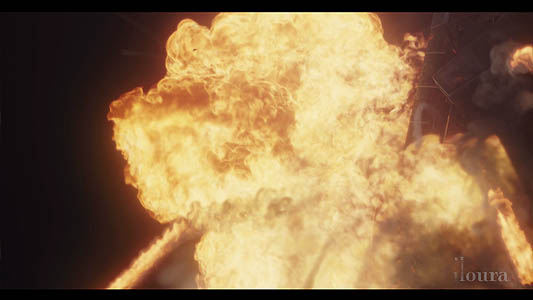
\includegraphics[width=\textwidth]{img/fumefx}
	\caption{Fire created with FumeFX~\cite{FumeFX}.}
	\label{fig:fumefx}
\end{figure}

\begin{figure}[htpb!]
        \centering
        \begin{subfigure}[t]{\textwidth}
                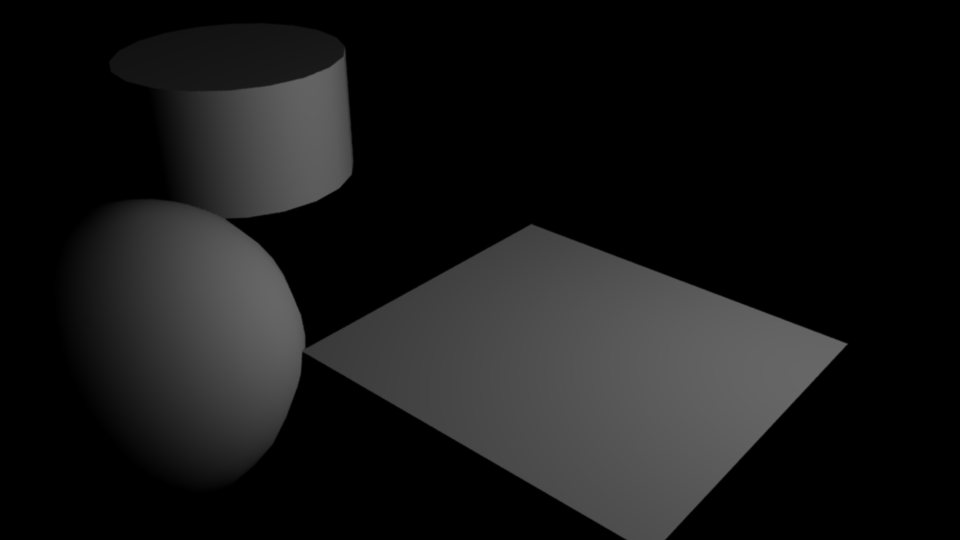
\includegraphics[width=\textwidth]{img/maya_no_fire_mental_ray}
                \caption{Scene without fire in \Maya, rendered with \MentalRay.}
                 \label{fig:maya_no_fire_mental_ray}
        \end{subfigure}    
        \\     
\end{figure}

\begin{figure}[htpb!]
		\ContinuedFloat
		\begin{subfigure}[t]{\textwidth}
                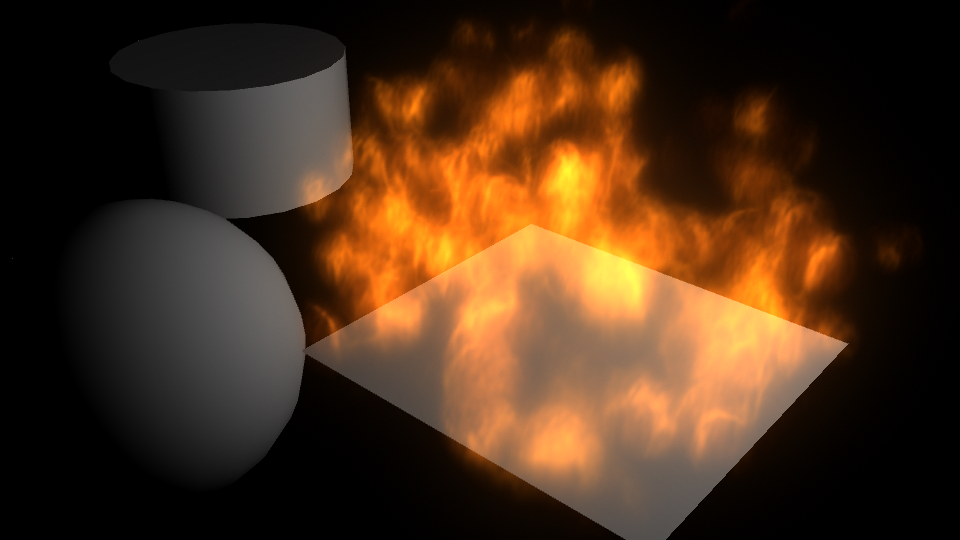
\includegraphics[width=\textwidth]{img/maya_fire}
                \caption{\Maya fire effect on a plane, rendered with \Maya software.}
                \label{fig:maya_fire}
        \end{subfigure}%        
\end{figure}

\begin{figure}[htpb!]
        \ContinuedFloat
 		\begin{subfigure}[t]{\textwidth}
                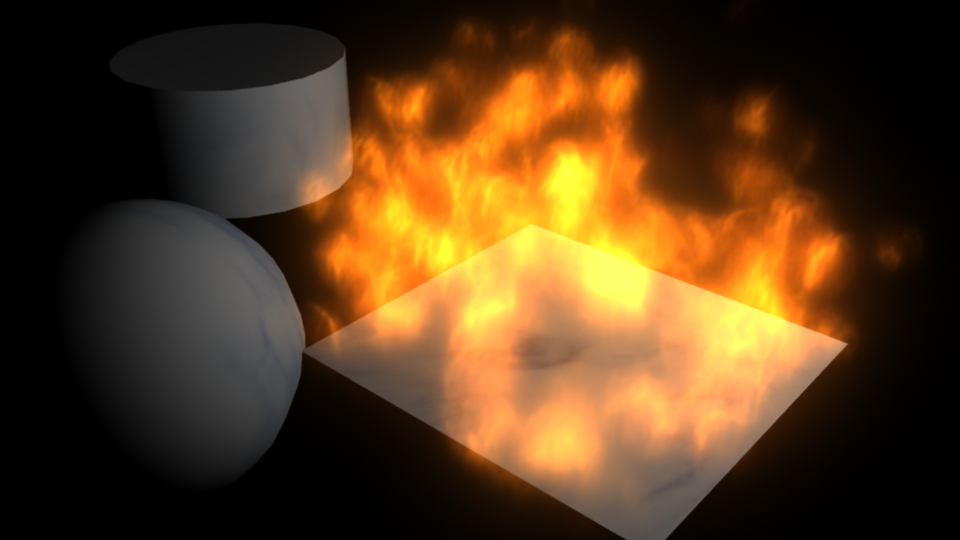
\includegraphics[width=\textwidth]{img/maya_fire_mental_ray}
                \caption{\Maya fire effect on a plane, rendered with \MentalRay.}
                \label{fig:maya_fire_mental_ray}
        \end{subfigure}%             
        \caption{Render tests for \Maya default fire effect.}
        \label{fig:maya_fire_scenes}
\end{figure}

\begin{figure}[htbp!]
	\centering
	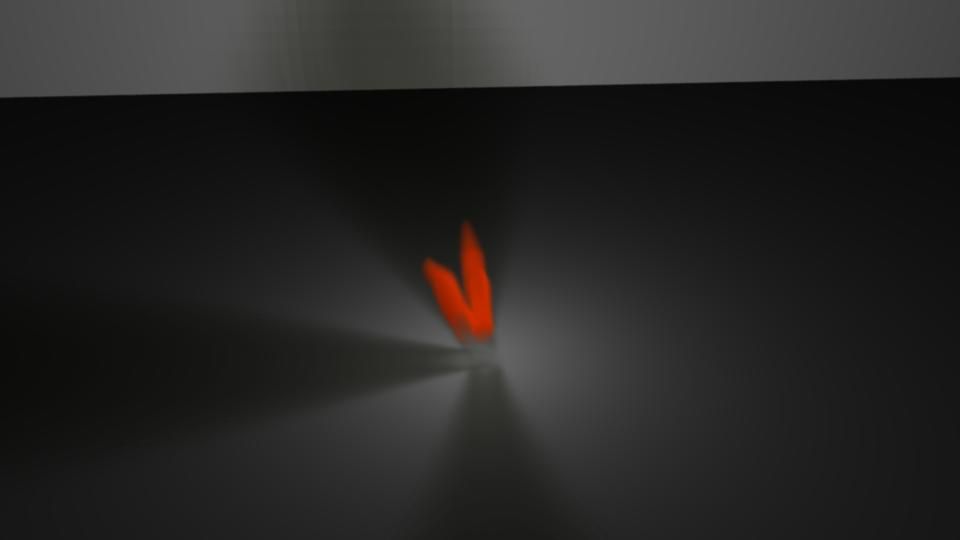
\includegraphics[width=\textwidth]{img/result_early_stage}
	\caption{Our renderer, early test, basic ray marching.}
	\label{fig:result_early_stage}
\end{figure}

\begin{figure}[htbp!]
	\centering
	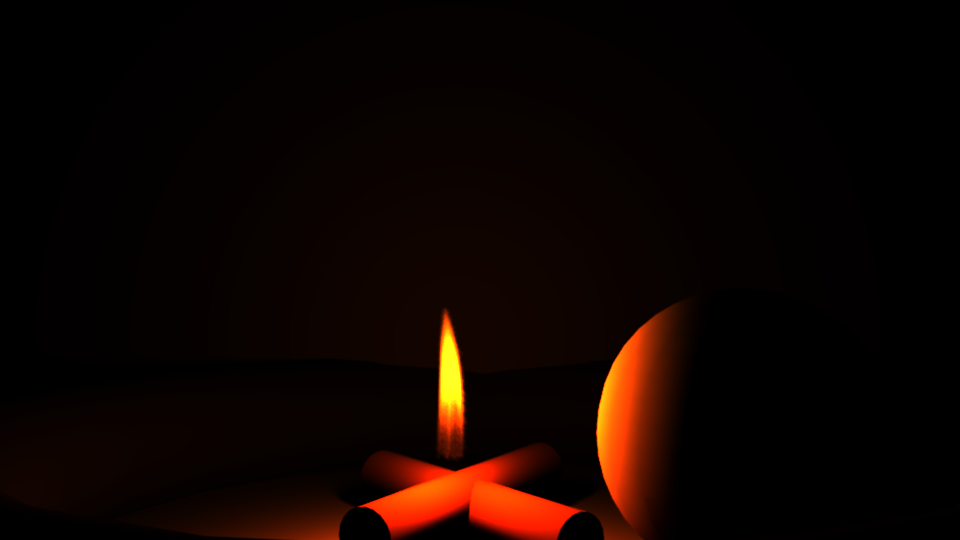
\includegraphics[width=0.8\textwidth, trim={8cm 0 8cm 10cm}, clip]{img/result_blackbody}
	\caption{result blackbody.}
	\label{fig:result_blackbody}
\end{figure}

\begin{figure}[htbp!]
	\centering
	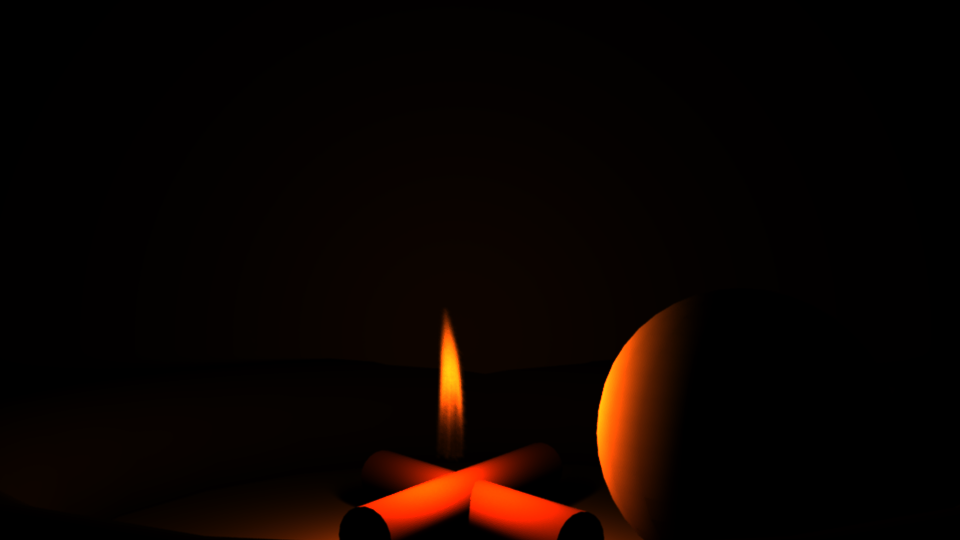
\includegraphics[width=0.8\textwidth, trim={8cm 0 8cm 10cm}, clip]{img/result_propane}
	\caption{result propane.}
	\label{fig:result_propane}
\end{figure}

\begin{figure}[htbp!]
	\centering
	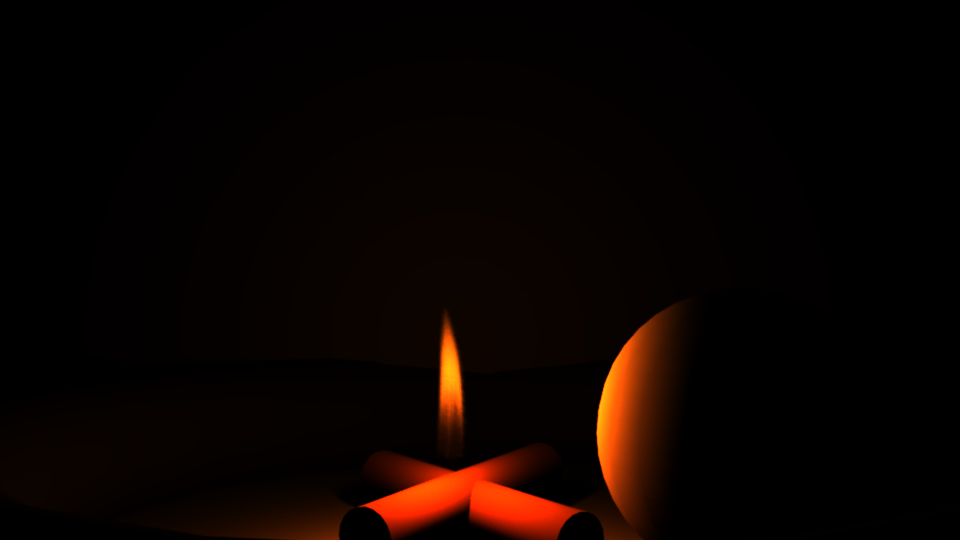
\includegraphics[width=0.8\textwidth, trim={8cm 0 8cm 10cm}, clip]{img/result_propane_shadows}
	\caption{result propane shadows.}
	\label{fig:result_propane_shadows}
\end{figure}

\begin{figure}[htbp!]
	\centering
	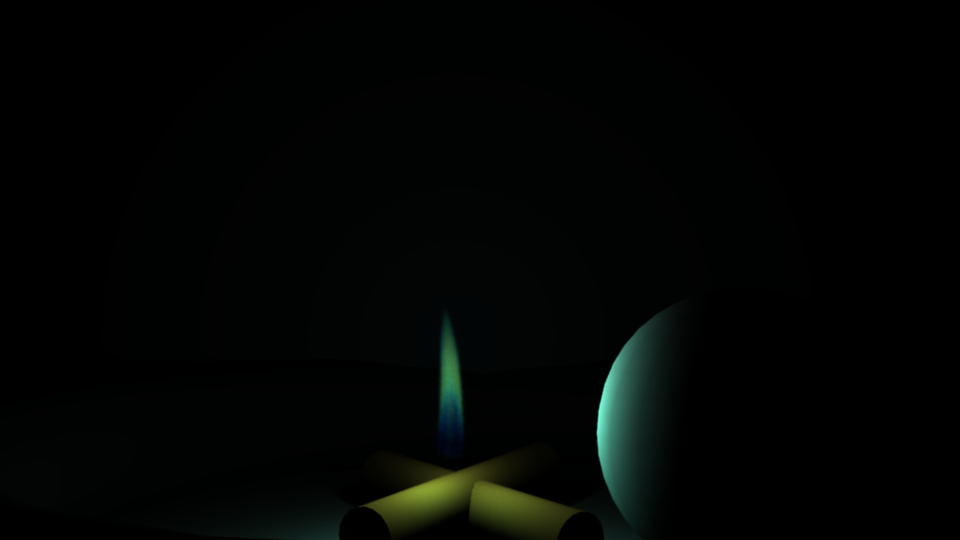
\includegraphics[width=0.8\textwidth, trim={8cm 0 8cm 10cm}, clip]{img/result_copper}
	\caption{result copper.}
	\label{fig:result_copper}
\end{figure}

\begin{figure}[htbp!]
	\centering
	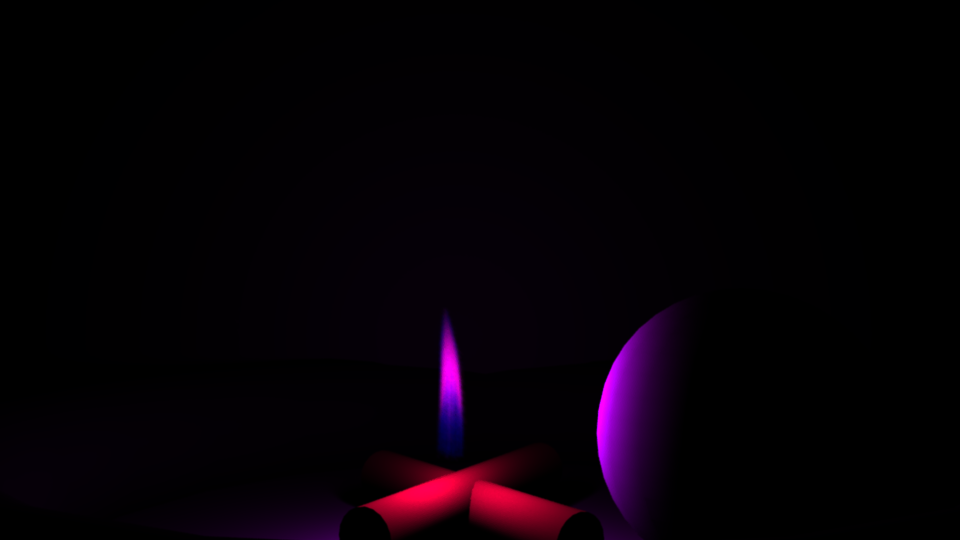
\includegraphics[width=0.8\textwidth, trim={8cm 0 8cm 10cm}, clip]{img/result_sulfur}
	\caption{result sulfur.}
	\label{fig:result_sulfur}
\end{figure}

\begin{figure}[htbp!]
	\centering
	
\includegraphics[width=0.25\textwidth]{img/result_synthetic}
	\caption{Our renderer, early test, basic ray marching.}
	\label{fig:result_synthetic}
\end{figure}

%------------------------------------------------------------------------------
\chapter{Conclusions and Future work}

\newpage
\bibliographystyle{apalike}
\bibliography{fire_rendering}

\end{document}

